\section{Projektplan}

\subsubsection{Zweck dieses Dokuments}
Dieses Dokument beschreibt den Projektplan des Projekts «Methode 635 als Cross Plattform App mit Xamarin». Es beinhaltet die Planung, die Organisation sowie weitere Aspekte und liefert damit eine gute Übersicht über das Projekt. Es dient daher als Grundlage für den Verlauf des Projekts.

\subsubsection{Gültigkeitsbereich}
Der Gültigkeitsbereich erstreckt sich über die gesamte Dauer des Projekts. Der Zeitraum geht vom 17. September 2018 bis zum 21. Dezember 2018. Das Projekt findet im Rahmen des Moduls «Studienarbeit» im Herbstsemester 2018 statt.

\subsection{Projektziel}
Die Motivation dieser Studienarbeit besteht darin, eine Cross-Platform App zu programmieren, welche die Methode 635 als mobile App für Android und iOS umsetzt. Dabei sollen moderne Technologien zum Einsatz kommen, welche es den Anwendern ermöglichen schneller und einfacher eine Lösung für ein Problem zu erarbeiten.

\subsubsection{Einschränkungen}
Das Projekt ist auf die Dauer des Herbstsemester 2018 begrenzt (bis 21. Dezember 2018). Zudem sollte das Projekt mit ungefähr 240 Arbeitsstunden (gesamthaft 480 Stunden) realisiert werden können. Bleibt am Ende Zeit über, werden optionale Features implementiert und als zusätzliche Funktionalität ergänzt.

\subsection{Projektorganisation}
In unserem Projekt arbeiten wir in einer flachen Organisationsstruktur, wobei die wesentlichen Entscheide, im ganzen Projektteam und/oder mit dem Dozenten an den wöchentlichen Meetings getroffen werden. An den Meetings getroffene Entscheidungen werden in Protokollen dokumentiert. Die Projektmitglieder sind innerhalb des Teams gleichgestellt.

\subsubsection{Organisationsstruktur}
% TODO Evtl. mit Bildern von uns und kurzer Beschreibung mit Namen und Funktion innerhalb des Teams

\subsubsection{Ansprechspartner}
Im Projekt «Methode 635 als Cross Plattform App mit Xamarin» sind folgende Ansprechpartner vorhanden.
% TODO Tabelle mit Angaben von Betreuer 

\subsection{Projektmanagement}
Eine ausführliche Iterationsplanung mit den dazugehörigen Meilensteinen befindet sich auf Jira. Die aufgewendeten Zeiten für ein Issue werden ebenfalls dort erfasst. 
Da wir mit einer agilen Entwicklung arbeiten, wird die Planung während dem Projekt laufend aktualisiert und den aktuellen Gegebenheiten angepasst. 
Nachfolgend ist jedoch schon ein grober Projektablauf ausgearbeitet. 

Zur Verwaltung des Codes nutzen wir öffentliche Github Repositories. Die Kommunikation abseits der HSR Anwesenheit erfolgt über einen Whats-App Chat.

% TODO Timeline einfügen

\subsubsection{Besprechungen}
Wenn immer möglich trifft sich einmal in der Woche das ganze Projektteam miteinander um sich über den aktuellsten Stand des Projekts auszutauschen, Fragen zu klären, Probleme anzugehen und die nächsten Schritte zu planen. 
Diese wöchentlichen Besprechungen finden jeden Donnerstagmorgen jeweils um 09:00 Uhr statt.
Über jede Besprechung wird Protokoll geführt. Dies mit
dem Ziel, die Entscheidungen festzuhalten und Missverständnisse zu vermeiden.

\subsubsection{Risikomanagement}
% TODO Excel File mit Risiken für das Projekt ausfüllen und einfügen

\subsubsection{Umgang mit Risiken}
Um auch auf unbekannte Risiken vorbereitet zu sein, wurde am Ende des Projektes eine Reserve eingeplant. Zudem haben Sie alle Teilnehmer bereit erklärt ihr Engagement punktuell zu erhöhen, falls die Situation dies erfordern würde. Diese Erhöhung sollte jedoch nur Phasenweise sein und in einer folgenden Phase kompensiert werden.

\subsubsection{Qualitätsmassnahmen}
Das Endprodukt dieses Projekts soll von möglichst hoher Qualität sein. Es wurden folgende Massnahmen getroffen um diese Qualität auch zu erreichen.

% TODO Liste mit Massnahme, Zeitraum, Ziel

\subsubsection{Eingesetzte Werkzeuge}
Die Entwicklungsumgebungen wurden so gewählt, dass Sie auf jedem Betriebssystem (Mac, Linux, Windows) eingesetzt werden können. Zudem wurde darauf geachtet, dass diese wenn möglich ohne Kosten verbunden sind. Die Entwicklungswerkzeuge unterscheiden sich je nach Entwicklungsbereich. Die folgende Tabelle gibt Auskunft über die eingesetzten Entwicklungsumgebungen.


\subsection{Entwicklung}
Der Entwicklungscode wird in öffentlichen Github Repositories unter unserer Gruppe https://github.com/BrainingOutOfBox gehalten. Für alle einzelnen Teile des Projekts gibt es ein eigenes Repository.

% TODO Liste mit Reponame und Link

\subsubsection{Vorgehen bei der Entwicklung}
Jedes Teammitglied verfügt über eine lokale Kopie der Repositories von Github. Für jede Aufgabe/Issue wird ein eigener Branch erstellt, unter Angabe der Nummer. Darin werden die Änderungen für diese Aufgabe vorgenommen. Die Änderungen sollen mit sinnvollen und präzisen Commit-Notizen festgehalten werden. Um ein Tracking der Änderung möglichst effizient zu gestalten, gilt es möglichst früh, möglichst viel zu commiten, sowie diese sinnvoll zu benennen.

\subsubsection{Code Guidelines}
Da Xamarin auf .Net bzw. C\# aufbaut, werden die Code Guidelines von .Net verwendet
% TODO .Net Guidelines: https://docs.microsoft.com/en-us/dotnet/standard/design-guidelines/

\subsection{Builden und testen der App}
Für das automatisierte Builden und Testen nach einem Commit wird auf Visual Studio App Center von Microsoft gesetzt. Zum Einen ermöglicht es eine einfache Integration von Github und zum Anderen bringt es alles mit, um Xamarin Apps automatisch zu builden, testen und deployen. 


\begin{landscape}
	\thispagestyle{empty}
	\subsection{Projektplan}
		\begin{figure}[h]
			\centering
			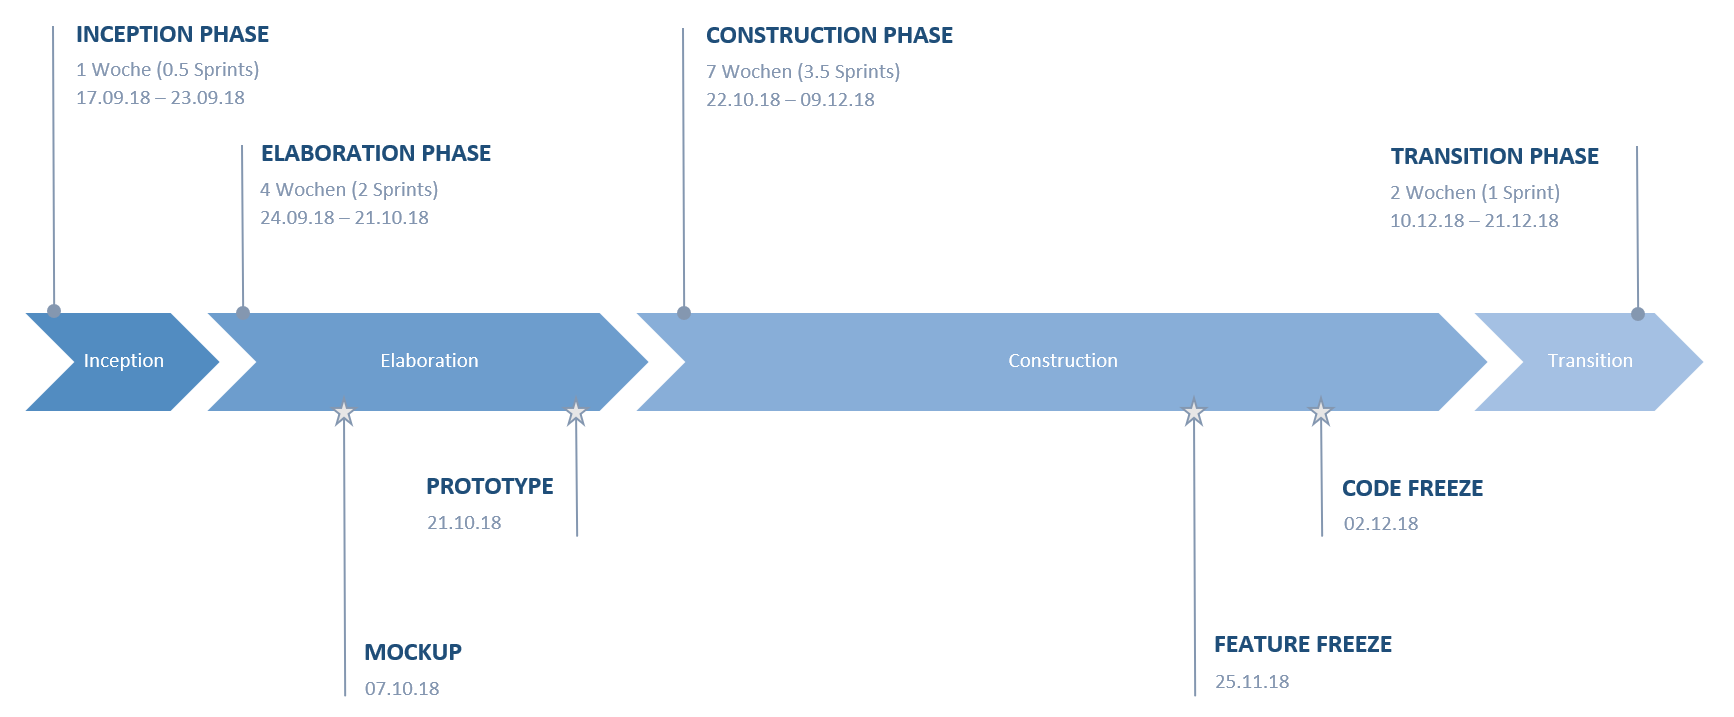
\includegraphics[width=1\linewidth, height=9.6cm]{img/projekt-plan/projekt-plan}
			\caption[Projektplan]{Projektplan}
			\label{fig:projekt-plan}
		\end{figure}
\end{landscape}